\documentclass[12pt,a4paper]{sprace} 
%###########################################################################
%%%%%%%%%%%%%%%%%%%%%  REPORT  %%%%%%%%%%%%%%%%%%%
%%%%%%%%%%%%%%%%% http://www.fapesp.br/176#4613 %%%%%%%%%%%%%%%
%###########################################################################
\usepackage[utf8]{inputenc}
\usepackage{url}
\usepackage{hyperref}
\hypersetup{pdftitle={Breno Orzari - Projeto de BEPE},
            pdfauthor={Breno Orzari, Thiago Rafael Fernandez Perez Tomei},
			colorlinks=true,
			citecolor=blue,
			linkcolor=black,
			urlcolor=blue			
           } % See http://en.wikibooks.org/wiki/LaTeX/Hyperlinks 
\usepackage{graphicx}
\usepackage[table]{xcolor}
\usepackage{tabularx}
%\usepackage[numbers,sort&compress]{natbib}
\usepackage[english]{babel}

\usepackage{booktabs}
\usepackage{topcapt}
\newcommand{\lin}{\color{spraceback}\rule{\linewidth}{0.8mm}}
\newcommand{\linha}{\enlargethispage{1\baselineskip}}    

%%% 2017, chega de usar baseline stretch!
%\renewcommand{\baselinestretch}{1.2}
\usepackage{setspace}
\onehalfspacing

\setlength\parindent{30pt}
% TITLE LINE
\usepackage{titlesec}
\titleformat{\section}
{\Large\sffamily}
{\thesection.}{.5em}{}[\color{spraceback}\titlerule]
%
%COLOR BOX
% http://tex.stackexchange.com/questions/66154/how-to-construct-a-coloured-box-with-rounded-corners
\usepackage{tcolorbox}% http://ctan.org/pkg/tcolorbox
\definecolor{spraceback}{HTML}{9F1F1B}   
\definecolor{spracetext}{HTML}{FFF8DC}   
\makeatletter
\newcommand{\mybox}[1]{%
  \setbox0=\hbox{#1}%
  \setlength{\@tempdima}{\dimexpr\wd0+13pt}%
  \begin{tcolorbox}[colframe=spraceback,colback=spraceback,boxrule=0.5pt,arc=4pt,
      left=6pt,right=6pt,top=6pt,bottom=6pt,boxsep=0pt,width=\@tempdima]
    #1
  \end{tcolorbox}
}
\makeatother


\newcommand{\alien}{\textit}
\newcommand{\Vz}{\cellcolor[gray]{1.0}\phantom{xxx}}
\newcommand{\LS}{\cellcolor{red!25}\phantom{xxx}}
\newcommand{\ST}{\cellcolor{blue!25}\phantom{xxx}}
\newcommand{\MT}{\cellcolor[gray]{0.75}\phantom{xxx}}
\newcommand{\LT}{\cellcolor{green!65!black}\phantom{xxx}}

\begin{document}

\begin{titlepage}

\begin{figure}[t] 

\includegraphics[height=2.25cm]{logoUNESP.pdf}
\hfill

\includegraphics[height=2.75cm]{logoSPRACE.png}
\end{figure}

\centering

\lin

\vspace{1.25cm}

{\LARGE Research Internship Abroad\\[1.0ex]
(Bolsa Estágio de Pesquisa no Exterior -- BEPE)} \\[1.25cm]

{\Large Machine Learning for Simulation\\[1.0ex]
of HEP Collisions with the CMS Detector}

\vspace{1.25cm}

\begin{minipage}{0.8\textwidth}
\textsf{
\begin{spacing}
{1.20}
\footnotesize
Summary goes here
\end{spacing}
}
\end{minipage}

\vfill
\lin
\flushright{{
\begin{tabular}{lr}
\textbf{Candidate:} & Breno Orzari\\
\textbf{Advisor in Brazil:} & Thiago R. F. P. Tomei\\
\textbf{Advisor Abroad:} & Maurizio Pierini\\
\textbf{Host Institution:}        & CERN\\
\end{tabular}
}}

%\lin
%\flushright{{\large
%\begin{tabular}{lr}
%Processo FAPESP:    & \textbf{2014/50208-0}\\
%\end{tabular}
%}}
\end{titlepage}


\tableofcontents
\clearpage

\section{Introduction}

%High Energy Physics (HEP) explores the elementary particles, which are the fundamental constituents of matter, and their interactions. Elementary particles are the underlying structure at the inner kernel of matter and, at the same time, plays an essential role in the evolution of the Universe. The last century has shown that collider accelerators have been among the most powerful tools used to explore the deep structure of matter that  enabled the development of a universal quantum field theory --- the standard model. HEP experiments led to important discoveries that go from the identification of heavy quarks, passing by the discovery of the W$^\pm$ and Z\textsuperscript{0} bosons, up to the breakthrough represented by the recent discovery of the Higgs boson at CERN~\cite{aad:2012tfa,Chatrchyan:2012xdj}, evidence for the Brout-Englert-Higgs mechanism through which fundamental particles acquire their mass.

The \emph{Large Hadron Collider} (LHC) at CERN~\cite{evans:2008zzb}, the most advanced high-energy physics (HEP) collider in operation, has opened new opportunities to explore the energy frontier of physics, colliding protons (pp) at a centre-of-mass energy of 13~TeV, which allows to explore distances as small as 10\textsuperscript{-18} meters. The LHC hosts two large general-purpose experiments, ATLAS (A Toroidal LHC ApparatuS)~\cite{Aad:2008zzm} and CMS (Compact Muon Solenoid)~\cite{chatrchyan:2008zzk}, operating on the Swiss-French border near Geneva, Switzerland. As of this writing, the LHC has just finished its second operation run (Run 2)~\cite{LHCEndRun2}, having delivered more than 150~fb\textsuperscript{-1} of 13~TeV pp collision data to both ATLAS and CMS.

The simulation, reconstruction and analysis of high-energy pp collisions, hereafter referred to as \emph{events}, are computer-intensive operations, which depend strongly on the complexity of the event in question. One particular aspect of the LHC operation is the occurrence of additional pp interactions in the same or neighbouring bunch crossings, referred to as pileup (PU). For the LHC Run 2 configuration, the average pileup $\langle \text{PU} \rangle$ observed was close to 40. The time required for reconstructing and/or simulate such an event reaches 1--10 minutes; with $\mathcal{O}(10^{10})$ events to be treated in that way, it is clear that not only a high-performance computing infrastructure is needed, but also time-effective algorithms.

In order to seize the opportunities and address the challenges posed by the ever-increasing LHC performance, the HEP field is moving closer to the frontier of information technology and computer science~\cite{Alves:2298968}. The new techniques, tools and frameworks from the field of \emph{machine learning} (ML) are ideally suited to the LHC era~\cite{Radovic2018}. The usage of ML techniques is not foreign to HEP; indeed, the ROOT data analysis framework has incorporated a Toolkit for Multivariate Analysis (TMVA) since 2013~\cite{TMVA}. Solutions based in machine learning have been extensively used in the LHC experiments, for identification of heavy-flavour jets~\cite{Sirunyan:2017ezt}, reconstruction and identification of $\tau$ leptons~\cite{Sirunyan:2018pgf}, energy reconstruction of electrons~\cite{Khachatryan:2015hwa} and even high-level physics studies like searches for resonant $t\overline{t}$~\cite{Sirunyan:2018ryr} and supersymmetric partners of the top quark~\cite{Sirunyan:2018omt}. The Deep Neural Networks (DNN) revolution~\cite{Goodfellow-et-al-2016} has, however, made significant impact on HEP; it is particularly promising when there are both a large amount of data and a high number of features, as well as symmetries hidden in the data and complex nonlinear dependencies between inputs and outputs, as is the case in HEP events.

The BEPE candidate, Mr. Breno Orzari, is currently working on a viability analysis of the search for dark matter with the CMS detector at the LHC, using the Dark Higgs model as a benchmark~\cite{Autran:2015mfa,Duerr:2017uap}. Usually, the simulation of the passage of particle sand radiation through the detector is achieved by the GEANT platform~\cite{agostinelli:2002hh} using Monte Carlo methods, but the time cost of such a simulation is prohibitive for such a preliminary study. He is using instead the Delphes~\cite{defavereau:2013fsa} framework for the fast simulation of the CMS detector; it employs a parameterised description of the interaction of the particles produced in the collision with the sensitive elements of the detector. The usage of Generative Adversarial Networks (GANs)~\cite{NIPS2014_5423} in the simulation of HEP events for that step has been studied for some time~\cite{Paganini:2017dwg}, with some very recent promising results on composite objects generation~\cite{Musella:2018rdi}. On the other hand, the usage of innovative architectures like graph neural networks in HEP problems has also been studied recently~\cite{Qasim:2019otl}, having inherent advantages like the absence of specific assumptions on the detector geometry. 

In this project, we propose an in-depth study of the suitability of ML techniques with graph networks for the simulation step. The candidate will work, together with their supervisor at CERN, on the development of a prototype simulator and compare with the results obtained using their current, Delphes-based setup.
 
\begin{figure}[t] %  figure placement: here, top, bottom, or page
   \centering
   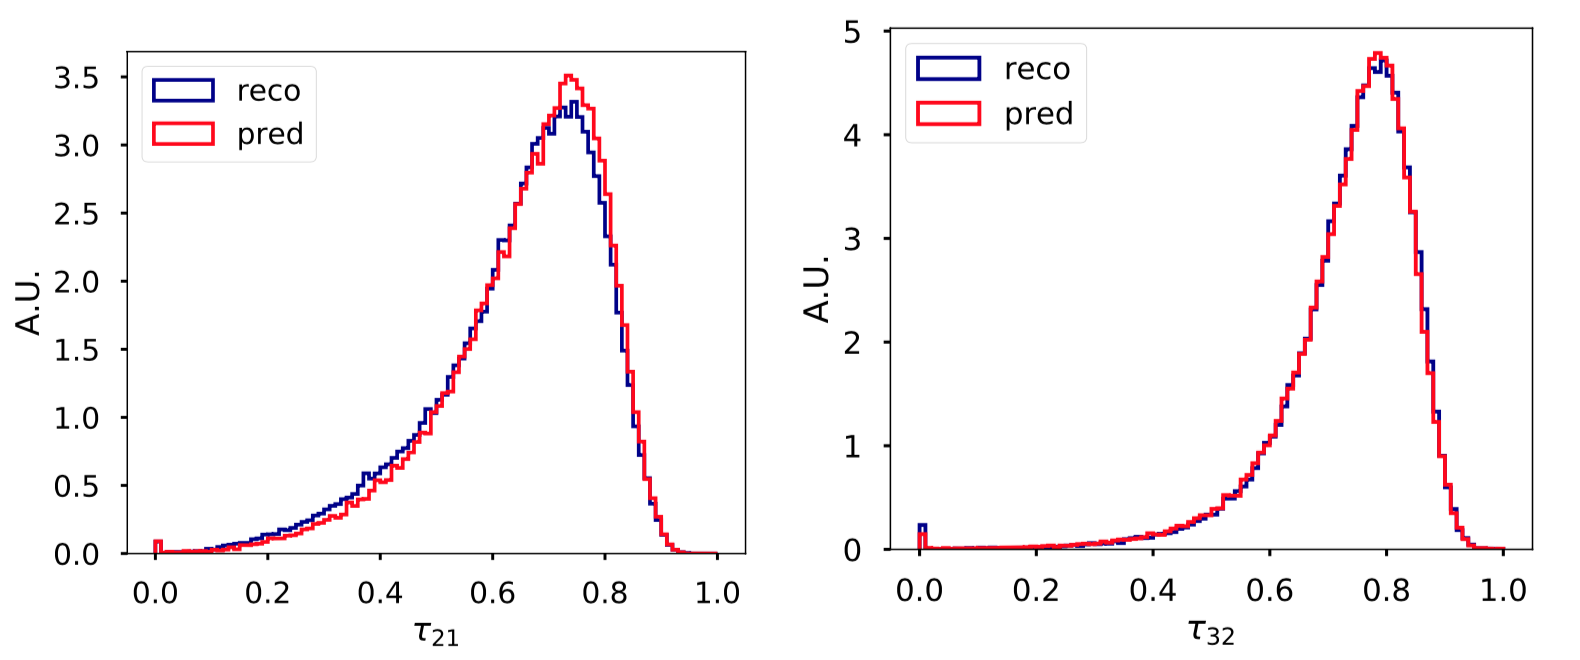
\includegraphics[width=0.95\textwidth]{GenerativeSubjettiness.png} 
   \caption{Distribution of high level variables used for discrimination between regular hadronic jets and ``merged jets'', like those coming from the decay of high-energy vector bosons. Blue histograms are obtained from the input data, while red ones are obtained using the generative model. Figure adapted from \cite{Musella:2018rdi}.}
   \label{fig:generativetau}
   \end{figure}

\clearpage

\section{Goals and Expected Results}

The goal of this project is for the student to learn the latest techniques and tools used in the development of algorithms for the simulation of the CMS detector, with emphasis on machine learning tools and particularly on graph neural networks. He will be working closely with the foremost experts in the subject, and with tools already adapted to the High Energy Physics environment, in order to get up to speed in a short time. He will go through all the steps of the algorithm development:
\begin{itemize}
\item Data formatting for the machine learning tools.
\item Definition of the event sets that make up the signal and background samples.
\item Choice, training and performance measurement of the ML models.
\item Efficiency and throughput parameterisation as function of event high-level quantities.
\end{itemize}

The expected result is that the student will develop a working knowledge on the usage of machine learning techniques, applied to the particular case of simulation of HEP events, as well as a set of simulated events that can be compared with the Delphes parameterisations. This comparison will, in turn, enrich his Masters' dissertation work, and at the same time lay the groundwork for him to work on those subjects at a deeper level for his Ph.D.

\clearpage
\section{Plan of Work and Project Execution Schedule}

\begin{table}[htbp]
\topcaption{Plan of work and schedule for the student.}
%\fontspec[Scale=0.85,Ligatures=TeX]{Helvetica}
%\singlespacing
\rule{0pt}{0.1\baselineskip}

\tiny
\centering
\begin{tabular}{|l|l|l|l|l|l|l|l|l|l|l|l|l|}
\hline
\textbf{Activities} & 
\textbf{Week 1} & \textbf{Week 2} & \textbf{Week 3} & \textbf{Week 4} &
\textbf{Week 5} & \textbf{Week 6} & \textbf{Week 7} & \textbf{Week 8}  &
\textbf{Week 9} & \textbf{Week 10} & \textbf{Week 11} & \textbf{Week 12}  \\
\hline
Data formatting & \MT & \MT & \Vz & \Vz & \Vz & \Vz & \Vz & \Vz & \Vz & \Vz & \Vz & \Vz\\
for ML tools.  	& \MT & \MT & \Vz & \Vz & \Vz & \Vz & \Vz & \Vz & \Vz & \Vz & \Vz & \Vz \\
\hline
Definition of signal and & \Vz & \MT & \MT & \MT &  \Vz &  \Vz & \Vz & \Vz &  \Vz &  \Vz & \Vz & \Vz \\
background samples.      & \Vz & \MT & \MT & \MT &  \Vz &  \Vz & \Vz & \Vz &  \Vz &  \Vz & \Vz & \Vz \\
\hline
Preliminary study and  & \Vz & \Vz & \MT & \MT &  \MT &  \Vz & \Vz & \Vz &  \Vz &  \Vz & \Vz & \Vz \\
choice of ML models.   & \Vz & \Vz & \MT & \MT &  \MT &  \Vz & \Vz & \Vz &  \Vz &  \Vz & \Vz & \Vz \\
\hline
Training of the   & \Vz & \Vz & \Vz  & \MT &  \MT &  \MT & \MT &  \MT &  \MT &  \Vz & \Vz & \Vz \\
ML models.        & \Vz & \Vz & \Vz  & \MT &  \MT &  \MT & \MT &  \MT &  \MT &  \Vz & \Vz & \Vz \\
\hline
Measurement of ML  & \Vz & \Vz & \Vz & \Vz & \MT &  \MT & \MT & \MT  & \MT & \MT & \Vz & \Vz \\
algo. performance. & \Vz & \Vz & \Vz & \Vz & \MT &  \MT & \MT & \MT  & \MT & \MT & \Vz & \Vz \\
\hline
Wrap-up, debriefing,& \Vz & \Vz & \Vz & \Vz & \Vz & \Vz & \Vz & \Vz &  \Vz &  \MT & \MT & \MT \\
final report.       & \Vz & \Vz & \Vz & \Vz & \Vz & \Vz & \Vz & \Vz &  \Vz &  \MT & \MT &\MT \\
\hline
\end{tabular}
\end{table}

\section{Materials and Methods}

The student will use the standard tools of High Energy Physics and Machine Learning for his studies, as follows:
\begin{itemize}
\item The standard combination of Pythia~\cite{sjostrand:2014zea} for the simulation of high-energy hadron collisions and GEANT for the simulation of the interaction of outgoing particles with the detector elements will be used. The implementation of the CMS detector geometry in GEANT is extremely complicated, therefore the prepackaged configurations available in the CMS Software suite (CMSSW)~\cite{ref:cmsswgithub} will be used. Those simulated events will comprise the reference sample against which the generative models will be validated.
\item The ROOT framework~\cite{brun:1996xxx} is the HEP standard, but the field is moving rapidly towards a convergence with Python-based packages that are the norm in the Computer Science field. The uproot package~\cite{pivarski2017uproot} allows for ROOT I/O in pure Python, creating an effective bridge between the two fields.
\item For the definition, training and evaluation of the Machine Learning models, the gold standard at the moment is the combination of the NumPy library for multi-dimensional arrays~\cite{numpy}, the Keras API for easy model construction~\cite{chollet2015keras}, and the TensorFlow backend for optimised computation~\cite{tensorflow2015-whitepaper}.
\end{itemize}

\clearpage

\section{Form of Analysis of Results}

In a complete analysis of the results of the CMS experiment, the observed data are compared with both standard model simulations and new physics signal simulations. This project has a reduced scope: only simulated data will be used to develop an algorithm capable of simulating the response of the CMS detector to the passage of particles coming from high-energy pp collisions, with high accuracy and throughput. The student will participate in the systematic design, implementation, training and evaluation of different models of GNNs, including the comparison with the GEANT-based reference sample.

The statistical analysis will be done with the traditional tools of the area -- hypothesis tests (null hypothesis $H_0$ vs. alternative hypothesis $H_1$), ROC curves (efficiency vs. fake rate), and the correlation matrix between the input variables. The platforms described in the previous section also include extremely complete statistical packages, in order to allow the student to perform this part of the analysis efficiently. At the end of the BEPE period, will describe his process and report and discuss his findings, making a comparison with the published literature.
\newpage\thispagestyle{empty}
\addcontentsline{toc}{section}{References}
\bibliography{ThiagoBib}{}

\end{document}